\documentclass[fullpage]{article}
\usepackage{tgpagella}
\usepackage{graphicx}
\usepackage{float}
\usepackage[english]{babel}
\usepackage[latin1]{inputenc}

\begin{document}

   \title{Experiment 4 - Building Topologies in NS3}

   \author{Muhammad Atif Farooq L144392 EE}

   \date{26th September 2019}

   \maketitle

\section{Introduction}
Carrier-Sense multiples access with collision avoidance or \textbf{CSMA} is a multiple
accesss channel method, where a multitude of nodes are connected to a common transmission
medium. The nodes then listen in on the traffic of the channel, trasmitting only when the
the channel is idle, in addition when they do transmit there packet load in full. It
is a protocol that appears in the Data Link Layer of the OSI model.

\section{Objective}
Build a network by making use of the \verb|CsmaHelper| class in NS3.

\section{Procedure}
For the lab task we were required to implement the following topology using the
\verb|CsmaHelper| class in NS3. We discuss the procedure by remarking first on the topology
in question and then discuss the stratedy we employed to realize this topology in NS3.

\begin{figure}[H]
  
\includegraphics[width=\linewidth]{topologyLabQuestion.png}
  \caption{topologyLabQuestion.png}
  \label{fig:output1}
\end{figure}

\subsection{The Topology}
As illustrated in the above figure we were required to implement two csma channels
i.e. bus topologies with there terminal nodes being connected by a point to point link.
nodes six and nodes two were meant to house the client and the server respectively, with
the server being configured to listen in on port 93.

\subsection{The Stratedgy Employed}
We started by first creating a node container to house the terminal nodes for the point to point
link we then created two other node container containing three nodes each, prepending one and
appending the second to the terminal nodes. The remaining task was the conventional NS3 procedure
of defining the channel attributes for the csma and point to point links, installing net devices
and protocols stack, assigning IPs, and installing the the server and client at the appropriate
nodes. We then enabled pcap tracing using the \verb|EnablePcap()| method of the \verb|CsmaHelper|
class to determine which of the nodes in the topology were involved in the routing process.

The required code and program output including the pcap traces are presented below.

\begin{verbatim}
  #include "ns3/core-module.h"
  #include "ns3/network-module.h"
  #include "ns3/csma-module.h"
  #include "ns3/internet-module.h"
  #include "ns3/point-to-point-module.h"
  #include "ns3/applications-module.h"
  #include "ns3/ipv4-global-routing-helper.h"

  using namespace ns3;

  NS_LOG_COMPONENT_DEFINE ("lab_question_script");

  int
  main (int argc, char *argv[])
  {
    // For verbose output and number of csma nodes.
    bool verbose = true;
    uint32_t nCsma = 3;

    CommandLine cmd;
    cmd.AddValue ("nCsma", "Number of \"extra\" CSMA nodes/devices", nCsma);
    cmd.AddValue ("verbose", "Tell echo applications to log if true", verbose);

    cmd.Parse (argc,argv);

    if (verbose)
      {
        LogComponentEnable ("UdpEchoClientApplication", LOG_LEVEL_INFO);
        LogComponentEnable ("UdpEchoServerApplication", LOG_LEVEL_INFO);
      }

    nCsma = nCsma == 0 ? 1 : nCsma;

    // Creating Node Container to House Nodes-0,1.
    NodeContainer p2pNodes;
    p2pNodes.Create(2);

    // Creating Node Container to House Nodes-1,2,3,4.
    NodeContainer csmaNodesOne;
    csmaNodesOne.Add(p2pNodes.Get(1));
    csmaNodesOne.Create(nCsma);

    // Creating Node Container to House Nodes-5,6,7,0.
    NodeContainer csmaNodesTwo;
    csmaNodesTwo.Create(nCsma);
    csmaNodesTwo.Add(p2pNodes.Get(0));

    // Specifying Point to Point Link Attributes.
    PointToPointHelper pointToPoint;
    pointToPoint.SetDeviceAttribute ("DataRate", StringValue ("5Mbps"));
    pointToPoint.SetChannelAttribute ("Delay", StringValue ("2ms"));

    // Installing Net Devices.
    NetDeviceContainer p2pDevices;
    p2pDevices = pointToPoint.Install (p2pNodes);

    // Specifying csma channel Attributes.
    CsmaHelper csmaOne;
    csmaOne.SetChannelAttribute ("DataRate", StringValue ("100Mbps"));
    csmaOne.SetChannelAttribute ("Delay", TimeValue (NanoSeconds (6560)));

    CsmaHelper csmaTwo;
    csmaTwo.SetChannelAttribute ("DataRate", StringValue ("100Mbps"));
    csmaTwo.SetChannelAttribute ("Delay", TimeValue (NanoSeconds (6560)));

    // Installing NetDevices.
    NetDeviceContainer csmaDevicesOne,csmaDevicesTwo;
    csmaDevicesOne = csmaOne.Install(csmaNodesOne);
    csmaDevicesTwo = csmaTwo.Install(csmaNodesTwo);

    // Installing Protocol Stack on p2pNodes and csma nodes.
    InternetStackHelper stack;

    stack.Install(csmaNodesOne);
    stack.Install(csmaNodesTwo);

    // Specifying IP Assignments for point to point nodes.
    Ipv4AddressHelper address;
    address.SetBase ("10.1.1.0", "255.255.255.0");

    Ipv4InterfaceContainer p2pInterfaces;
    p2pInterfaces = address.Assign (p2pDevices);

    // Specifying IP Assignments for csma nodes.
    address.SetBase ("10.1.2.0", "255.255.255.0");
    Ipv4InterfaceContainer csmaInterfacesOne;
    csmaInterfacesOne = address.Assign (csmaDevicesOne);

    address.SetBase ("10.1.3.0", "255.255.255.0");
    Ipv4InterfaceContainer csmaInterfacesTwo;
    csmaInterfacesTwo = address.Assign (csmaDevicesTwo);

    // Creating Server on Node-3 with port 93 and Installing Server Apps.
    UdpEchoServerHelper echoServer (93);

    ApplicationContainer serverApps = echoServer.Install(csmaNodesOne.Get(nCsma-1));
    serverApps.Start (Seconds (1.0));
    serverApps.Stop (Seconds (10.0));

    // Creating Client on Node-2
    UdpEchoClientHelper echoClient (csmaInterfacesOne.GetAddress (nCsma-1), 93);
    echoClient.SetAttribute ("MaxPackets", UintegerValue (1));
    echoClient.SetAttribute ("Interval", TimeValue (Seconds (1.0)));
    echoClient.SetAttribute ("PacketSize", UintegerValue (1024));

    ApplicationContainer clientApps = echoClient.Install (csmaNodesTwo.Get (1));
    clientApps.Start (Seconds (2.0));
    clientApps.Stop (Seconds (10.0));

    // To Enable Routing.
    Ipv4GlobalRoutingHelper::PopulateRoutingTables ();

    // For tcp-dump traces of client and server.
    csmaOne.EnablePcap ("client", csmaDevicesOne.Get (1), true);
    csmaTwo.EnablePcap ("server", csmaDevicesTwo.Get (2), true);

    Simulator::Run();
    Simulator::Destroy();
    return 0;
  }
\end{verbatim}

\begin{figure}[H]
  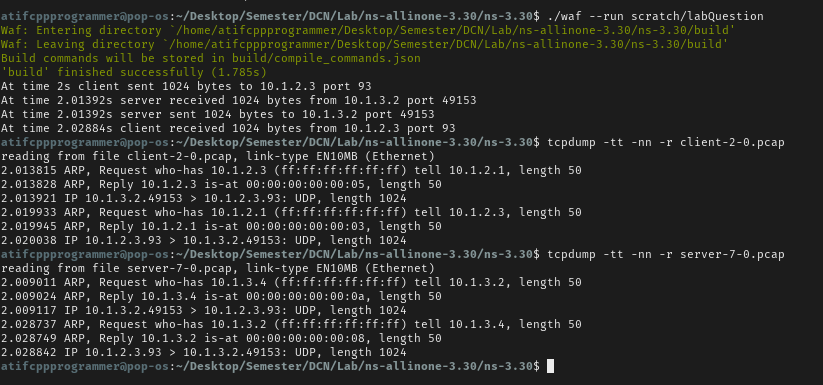
\includegraphics[width=\linewidth]{labQuestion.png}
  \caption{labQuestion.cc}
  \label{fig:output2}
\end{figure}

\section{Conclusions}
The \verb|CsmaHelper| class can used to create complex topologies that
incorporate bus topologies in NS3.

\section{Post-Lab Question}
For the post lab we werer required to implement the following topology.

\begin{figure}[H]
  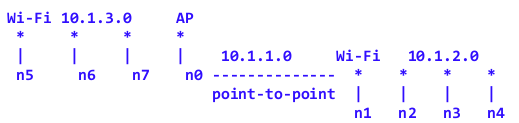
\includegraphics[width=\linewidth]{topologyPostLabQuestion.png}
  \caption{topologyPostLabQuestion.png}
  \label{fig:output2}
\end{figure}

The code required to implement the topology in question is presented in
\verb|examples/tutorial/third.cc| therefore we only provide the code required to
meet stipulations set in the statement of post lab question.

\begin{verbatim}
  UdpEchoServerHelper echoServer (93);

  ApplicationContainer serverApps = echoServer.Install (csmaNodes.Get (2));
  serverApps.Start (Seconds (1.0));
  serverApps.Stop (Seconds (10.0));

  UdpEchoClientHelper echoClient (csmaInterfaces.GetAddress (2), 93);
  echoClient.SetAttribute ("MaxPackets", UintegerValue (1));
  echoClient.SetAttribute ("Interval", TimeValue (Seconds (1.0)));
  echoClient.SetAttribute ("PacketSize", UintegerValue (1024));

  ApplicationContainer clientApps =
    echoClient.Install (wifiStaNodes.Get (1));
  clientApps.Start (Seconds (2.0));
  clientApps.Stop (Seconds (10.0));
\end{verbatim}

What follows are the script output in addition to the pcap traces of the point to
point nodes of the topology in question.

\begin{figure}[H]
  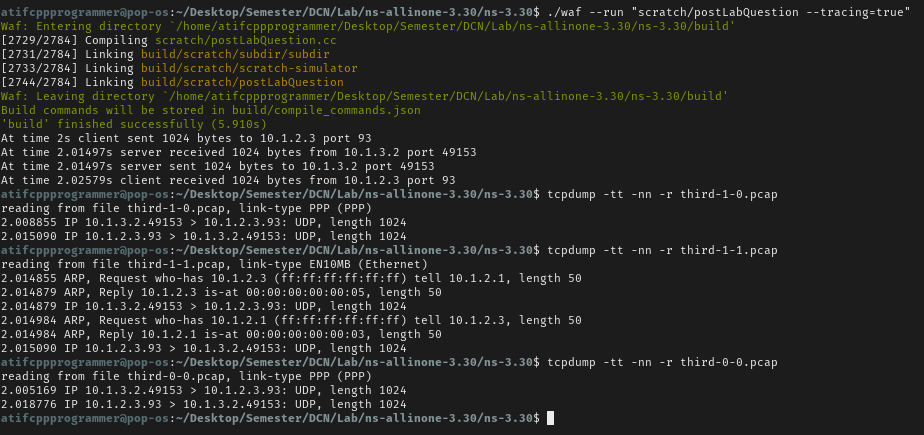
\includegraphics[width=\linewidth]{postLabQuestionOne.png}
  \caption{postLabQuestionOne.png}
  \label{fig:output3}
\end{figure}

\begin{figure}[H]
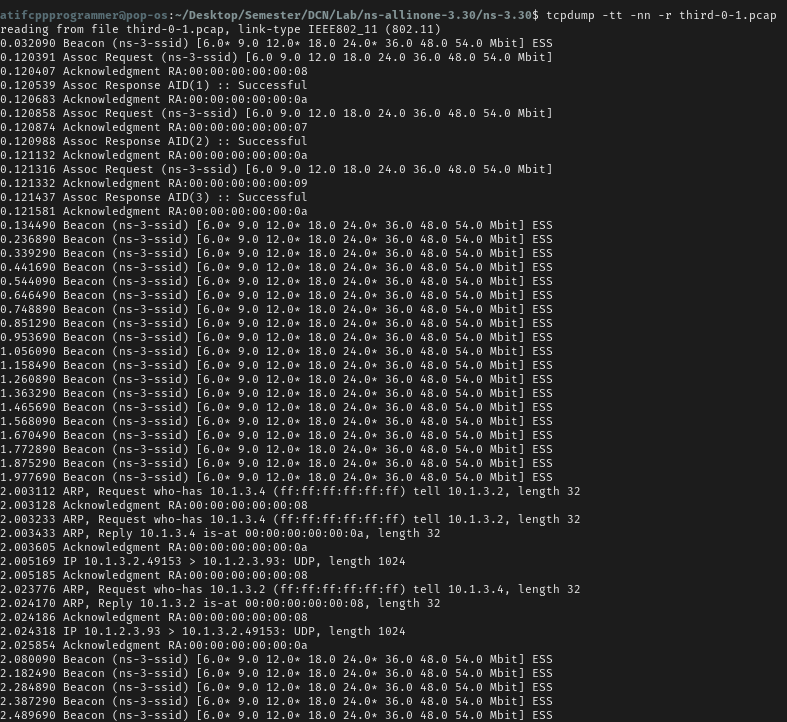
\includegraphics[width=\linewidth]{postLabQuestionTwo.png}
\caption{postLabQuestionOne.png}
\label{fig:output3}
\end{figure}

\end{document}
